\documentclass[10pt,letterpaper]{article} % {{{
\usepackage[utf8]{inputenc}
\usepackage[spanish]{babel}
\usepackage{amsmath}
\usepackage{amsfonts}
\usepackage{amssymb}
\usepackage{graphicx}
\graphicspath{{tmp/}}
\usepackage{physics}
\usepackage{bbm}
\usepackage[dvipsnames]{xcolor}
\usepackage[margin=1in]{geometry}
\usepackage{booktabs}
\usepackage{float}

\newcommand{\eref}[1]{eq.~(\ref{#1})} 
\newcommand{\sref}[1]{sec.~\ref{#1}}
\newcommand{\fref}[1]{Fig.~\ref{#1}}
\newcommand{\tref}[1]{table~\ref{#1}}
\newcommand{\Eref}[1]{Eq.~(\ref{#1})} 
\newcommand{\Sref}[1]{Sec.~\ref{#1}}
\newcommand{\Fref}[1]{Fig.~\ref{#1}}  
\newcommand{\Tref}[1]{Table~\ref{#1}}

\usepackage{hyperref}
\hypersetup{
colorlinks=true,
linkcolor=blue,
filecolor=blue,      
citecolor=blue,
urlcolor=blue,
pdftitle={},
pdfauthor=author={Jose Alfredo de Leon},
}

\usepackage{tikz}

\usepackage[mathlines]{lineno}  \linenumbers \setlength\linenumbersep{5pt}
\usepackage[inline]{showlabels,rotating}
\renewcommand{\showlabelrefline}{\hrule width 0pt height 3ex depth 0pt}
\renewcommand{\showlabelfont}{\small\slshape\color{red!70}}
\usepackage[draft,inline,nomargin]{fixme} \fxsetup{theme=color}
\definecolor{jacolor}{RGB}{200,40,0} \FXRegisterAuthor{ja}{aja}{\color{jacolor}JA}
\FXRegisterAuthor{cp}{acp}{\color{blue}CP}
\FXRegisterAuthor{cd}{acd}{\color{purple}CD}

\decimalpoint

\newcommand{\one}{\mathbbm{1}}

\newtheorem{theorem}{Teorema}
\newtheorem{proof}{Demostración}
\newtheorem{hypothesis}{Hipótesis}

\title{Quantum billiards and DTQW}
\author{Jose Alfredo de Leon}
\date{Última actualización: \today}

\renewcommand{\labelenumii}{\arabic{enumi}.\arabic{enumii}}
\renewcommand{\labelenumiii}{\arabic{enumi}.\arabic{enumii}.\arabic{enumiii}}
\renewcommand{\labelenumiv}{\arabic{enumi}.\arabic{enumii}.\arabic{enumiii}.\arabic{enumiv}}

\newcommand{\rhoel}[2]{\rho_{#1,#2} \dyad{#1}{#2}}
\newcommand{\p}{p_{\text{error}}}


\begin{document}
\maketitle

\section{Resumen}
En la Ref.~\cite{alonso-lobo_2025_simplest} implementan una DTQW 2D dentro 
de un estadio de Bunimovich y argumentan que las señales de caos están presentes. 
No obstante, en la $P(s)$ no se ve tan claro. Yo tengo intuición de que el sistema 
tiene que ser caótico, entonces creo que hay un problema con el unfolding 
o simetrías. De hecho, ni en el billar rectangular la $P(s)$ es una distribución 
de Poisson.

\section*{Notación que uso en estas notas}
\begin{itemize}
\item $(m,n) \longmapsto (x,y)$
\item $m_c \longmapsto x_c$
\item $m_u \longmapsto y_u$
\item $m_r \longmapsto x_r$
\end{itemize}

\section{Distribución de las proporciones de los espaciamientos $P(r)$}
Supongamos que la $P(s)$ no sale bien por el unfolding, entonces sería mejor 
revisar la $P(r)$~\cite{atas_2013_distribution} para no tener que hacer unfolding.  
En la Fig.~\ref{fig:1} se muestra el segundo caso que toman en el paper y se ve 
claro que se cumple la predicción de RMT. En el primer caso el  promedio 
del espaciamiento de niveles de indeterminado, por lo que creo que hay
unas simetrías que no están viendo en el paper. Es decir, incluso aunque hicieran 
un buen unfolding, creo que no verían nada con la $P(s)$ porque hay que separar
por simetrías.

\begin{figure}
\centering
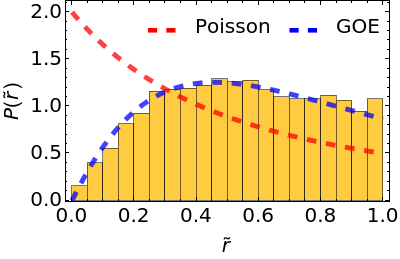
\includegraphics[width=0.7\textwidth]{Uv2_xc_50_alpha_Pi-4_beta_Pi-3.png}
\caption{Monedas de la v2 del arxiv~\cite{alonso-lobo_2025_simplest}. 
Dimensiones del estadio:
$\alpha=\pi / 4$, $\beta=\pi / 3$. $x_c = 50$, $x_r=2 x_c$ y $y_u = x_c$.}
\label{fig:1}
\end{figure}

\bibliographystyle{unsrt}
\bibliography{referencias.bib}
\end{document}